\chapter{Introduction} \label{chap:intro}

\section*{}

This first chapter aims to provide the reader with an overview of this
dissertation. It starts by introducing the context this work is inserted in,
identifying the problem which we aim to solve, how we plan on solving it, and
the expected outcome. Lastly, it gives a bird's eye view of this report's
structure.

\iffalse
O primeiro capítulo da dissertação deve servir para apresentar o
enquadramento e a moti\-va\-ção do trabalho e para identificar e
definir os problemas que a dissertação aborda.
Deve resumir as metodologias utilizadas no trabalho e termina
apresentando um breve resumo de cada um dos capítulos
posteriores.

Este documento ilustra o formato a usar em dissertações na \Feup, não
servindo de exemplo sobre os conteúdos a usar.
São dados exemplos de margens, cabeçalhos, títulos, paginação, estilos
de índices, etc.
São ainda dados exemplos de formatação de citações, figuras e tabelas,
equações, referências cruzadas, lista de referências e índices.

Uma recolha de normas existentes sobre este assunto pode ser
encontrada em~\cite{kn:Mat93}.

\begin{quote}
  ``Like the Abstract, the Introduction should be written to engage the
  interest of the reader. It should also give the reader an idea of
  how the dissertation is structured, and in doing so, define the
  thread of the contents.''~\cite[chap.\ Introduction]{kn:Tha01}
\end{quote}

Neste primeiro capítulo ilustra-se a utilização de citações e de
referências biblio\-grá\-fi\-cas.
Para além de dar um exemplo de utilização de uma citação, a citação
anterior, introduz uma referência que pode ser consultada, entre
muitas outras referências bibliográficas
interessantes~\cite{kn:Tha01,kn:PP05}.
\fi

\section{Context} \label{sec:context}

There is, among several domains with interesting and relevant problems to solve
(computer vision \cite{Kulkarni2015}, cryptography, biology, fraud detection,
recommender systems \cite{intml}, …), the recurring necessity to be able to
make decisions in the face of uncertainty using machine learning (ML) methods.

Successful ML applications include Google's personalized advertising and
context-driven information retrieval, Facebook's studies of how information
spreads across a network or UC Berkeley's AMPLab contributions towards Amazon
Web Service and SAP's products \cite{Broder:2015:BDN:2684822.2697027}.

Typically, there are two approaches for this class of problems): either use an
existing machine learning model (such as KNN, neural networks or similar) \cite{mlnot} and
try to fit your data into the model, or build a probabilistic model for your
particular problem so you can leverage domain knowledge \cite{SciPy}.

In the second approach one common way to tackle it is to use bayesian reasoning,
where you model unknown causes with random variables, feed the model the data you
have gathered and then perform inference to reverse the story and query for the
desired variables \cite{thbay}. The tricky issue is this last step, since it is non-trivial
to write an inference method \cite{Duvenaud}.

The solution to this has been building generic inference engines for graphical
models, so that modeling and inference can be treated as separate concerns and
people can focus on the modeling \cite{Jordan1996}. However, not all models can be represented as
graphical models, and that’s why we now have Probabilistic Programming Languages
(PPLs). Probabilistic Programs let you write your model as a program and have
off-the-shelf inference \cite{Prekopa2003}.

\section{Problem} \label{sec:proj}

In spite of these examples of applications in the industry, ML has been
identified by Gartner, in its Hype Cycle annual review,
to be in the "Peak of Inflated Expectations" stage, still far
from the "Plateau of Producitvity" \cite{gartner}.

It has also been said that ML's applications are rarely seen
outside the academia, with Wagstaff claiming that there is a "frequent lack of
connection between machine learning research and the larger world of scientific
inquiry and humanity" \cite{Wagstaff2012}.

Arguably the scenario is even worse for PPLs, having even lesser adoption
among tech companies. One factor which may be contributing to this lack of
usage, despite PP's power and flexibility, is the difficulty for data scientists
to adapt to textual interface these languages provide, which lack the graphical
intuiton provided by other tools they are accustomed to. In a poll made to about 2800
data scientists (see Figure \ref{fig:poll}), half of the top 10 tools are
graphically-interactable.

\begin{figure}[t]
  \begin{center}
    \leavevmode
    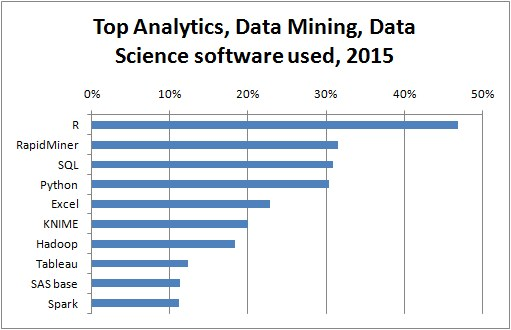
\includegraphics[width=0.86\textwidth]{poll}
    \caption{Top 10 Analytics Tools \cite{kdn}}
    \label{fig:poll}
  \end{center}
\end{figure}

\section{Motivation and Goals} \label{sec:goals}

DARPA, one of the funders behind PPLs' research, has recognized some of the problems
identified by Wagstaff and started a program called Probabilistic Programming
for Advancing Machine Learning (PPAML) to address the shortcomings of
current ML methods \cite{darpa}. It identifies five strategic goals:

\begin{itemize}
  \item Shorten machine learning model code to make models faster to write and
  easier to understand
  \item Reduce development time and cost to encourage experimentation
  \item Facilitate the construction of more sophisticated models that
  incorporate rich domain knowledge and separate queries from underlying code
  \item Reduce the level of expertise necessary to build machine learning
  applications
  \item Support the construction of integrated models across a wide variety of
  domains and tool types
\end{itemize}

The aim of this work is to try address
the first four. In order to do so, we will try to combine Visual Programming
(VP)

To address this issue, this dissertation aims to explore graphical
representations of a PPL through node-based programming.
This means having a visual editor that compiles what is drawn to a PPL’s syntax.
By being similar to other data analysis tools, such as RapidMiner or
Weka Knowledge Flow, we hypothesize it will be more intuitive and thus easier
to learn than a full-blown PPL.

\section{Estrutura da Dissertação} \label{sec:struct}

Para além da introdução, esta dissertação contém mais x capítulos.
No capítulo~\ref{chap:sota}, é descrito o estado da arte e são
apresentados trabalhos relacionados.
%\todoline{Complete the document structure.}
No capítulo~\ref{chap:chap3}, ipsum dolor sit amet, consectetuer
adipiscing elit.
No capítulo~\ref{chap:chap4} praesent sit amet sem.
No capítulo~\ref{chap:concl}  posuere, ante non tristique
consectetuer, dui elit scelerisque augue, eu vehicula nibh nisi ac
est.
